\section{Interrupt Performance}

\subsection{Event Detection Methods}

\begin{concept}{Event Detection in Embedded Systems}\\
    Peripherals Signal Events to Firmware: something happened that requires servicing firmware\\
    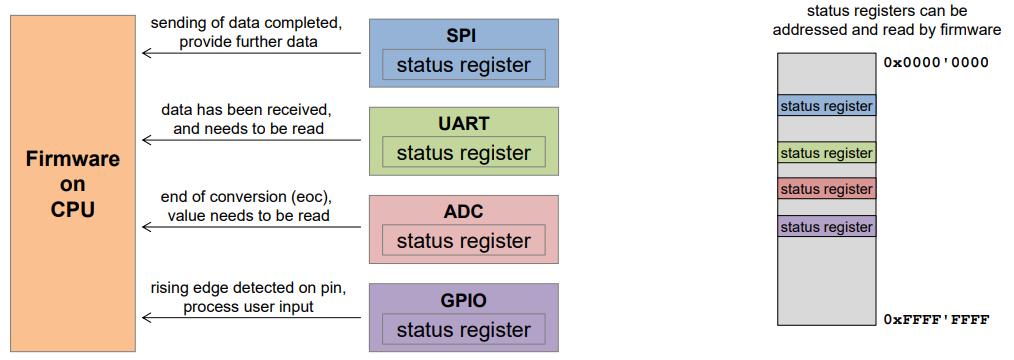
\includegraphics[width=\linewidth]{eventdetection.png}
\end{concept}

\subsubsection{Polling vs. Interrupt-Driven I/O}
Two primary methods for detecting events in embedded systems:

\begin{minipage}{0.38\linewidth}

\begin{concept}{Polling}\\  Periodically checking status registers
    \begin{itemize}
        \item Simple and straightforward
        \item Synchronous with main program (implicit synchronization)
        \item Predictable timing (deterministic)
        \item Simple implementation (no additional interrupt logic)
        \item Wastes CPU time (busy wait)
        \item Reduced throughput and long reaction times
    \end{itemize}
\end{concept}
\end{minipage}
\begin{minipage}{0.62\linewidth}
\begin{concept}{Interrupt-Driven I/O}
 Hardware signals CPU when events occur
    \begin{itemize}
        \item Asynchronous with main program
        \item CPU notified only when an event happens (efficient CPU utilization)
        \item Main program can focus on primary tasks
        \item Event-driven approach (good for infrequent, time-critical tasks)
        \item More complex implementation
        \item Can introduce timing uncertainties (non-deterministic behavior)
        \item Potential for interrupt conflicts and priority issues
        \item Overhead for context switching
    \end{itemize}
\end{concept}
\end{minipage}

\begin{definition}{Interrupt-Driven I/O}
In interrupt-driven I/O, peripherals notify the CPU when events occur:
\begin{itemize}
    \item Peripherals assert interrupt signal when they need servicing
    \item CPU temporarily suspends current execution
    \item Control transfers to an Interrupt Service Routine (ISR)
    \item After handling the interrupt, control returns to previous execution
\end{itemize}

Extreme case: All processing done in Interrupt Service Routines (ISR):\\
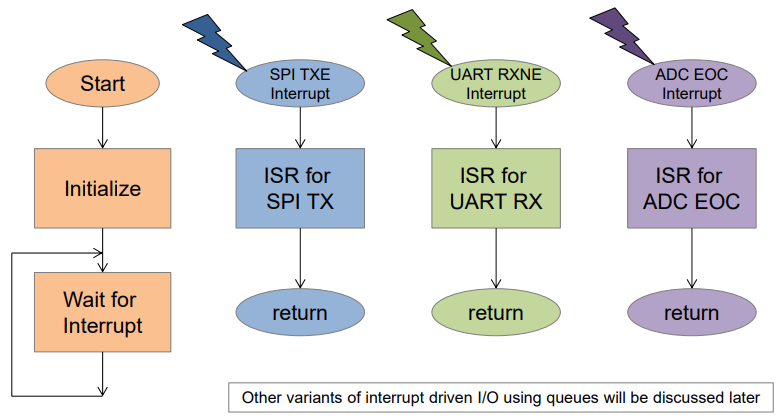
\includegraphics[width=0.8\linewidth]{interruptdrivenio.png}

\end{definition}

\subsubsection{Polling}

\begin{theorem}{Polling Implementation}
In polling, the CPU periodically checks status registers to detect events:
\begin{itemize}
    \item Main loop continuously or periodically inspects peripheral status
    \item When an event is detected, appropriate handler executes
    \item After handling, control returns to polling loop
    \item CPU always actively checking, even when no events occur
\end{itemize}
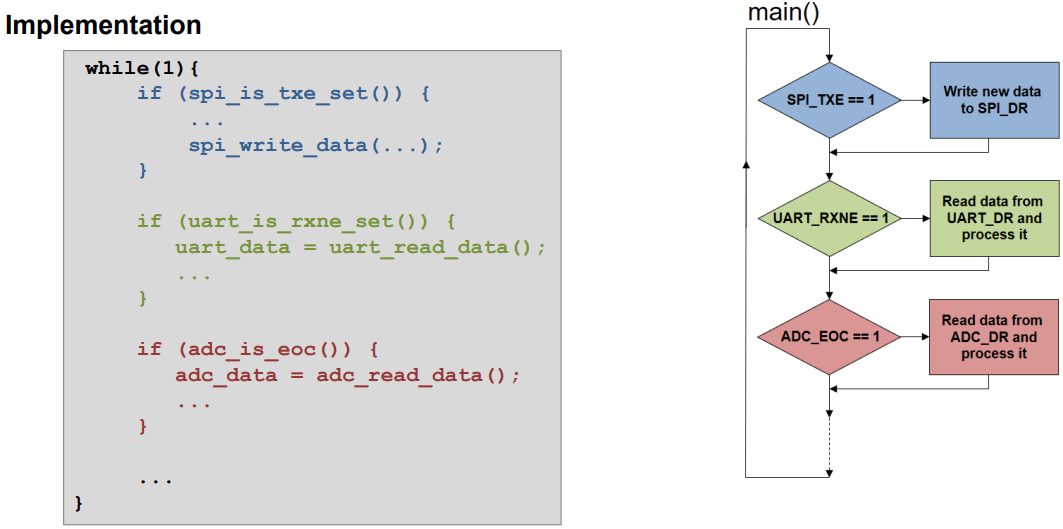
\includegraphics[width=0.8\linewidth]{polling_imple.png}
\end{theorem}



\begin{KR}{Implementing Polling in C}
\paragraph{Step 1: Identify status registers}
Determine which peripheral registers contain status information.
\paragraph{Step 2: Create a polling loop}
Implement a loop that regularly checks the status flags.
\paragraph{Step 3: Check for events}
Test specific bits in the status registers to detect events.
\paragraph{Step 4: Handle detected events}
Process events when their status flags are set.
\paragraph{Step 5: Clear status flags}
Reset status flags to prepare for next event detection.

\begin{lstlisting}[language=C, style=basesmol]
// Main polling loop
while (1) {
    // Check SPI transmit buffer empty flag
    if (SPI1->SR & SPI_SR_TXE) {
        // Handle SPI transmission
        if (spi_tx_count < spi_tx_length) {
            SPI1->DR = spi_tx_buffer[spi_tx_count++];
        }
    }
    // Check UART receive data register not empty flag
    if (USART2->SR & USART_SR_RXNE) {
        // Handle UART reception
        uint8_t data = USART2->DR;
        process_uart_data(data);
    }
    // Check ADC end of conversion flag
    if (ADC1->SR & ADC_SR_EOC) {
        // Handle ADC conversion complete
        uint16_t adc_value = ADC1->DR;  // Reading DR clears EOC flag
        process_adc_data(adc_value);
    }
    // Other system tasks
    process_system_tasks();
}
\end{lstlisting}
\end{KR}

\raggedcolumns
\columnbreak

\subsubsection{Interrupt-Driven I/O}

\begin{definition}{Interrupt System STMF32429I}\\
    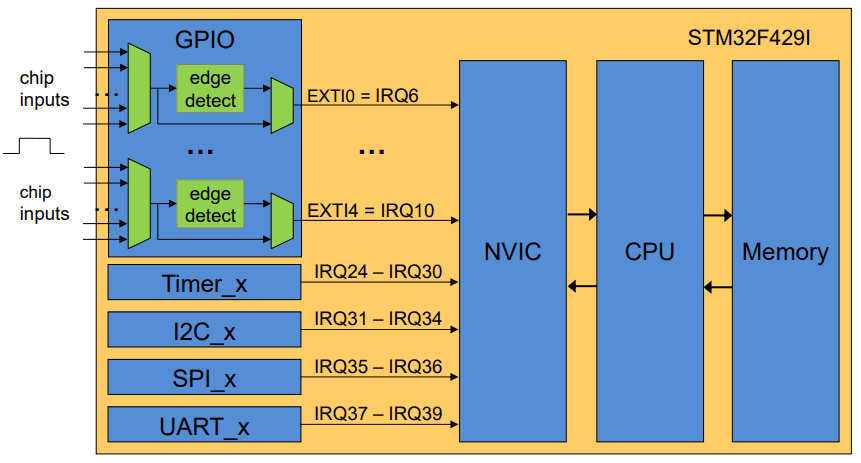
\includegraphics[width=0.7\linewidth]{interruptsystemstm.png}
\end{definition}

\begin{concept}{Vector Table and ISR}\\
    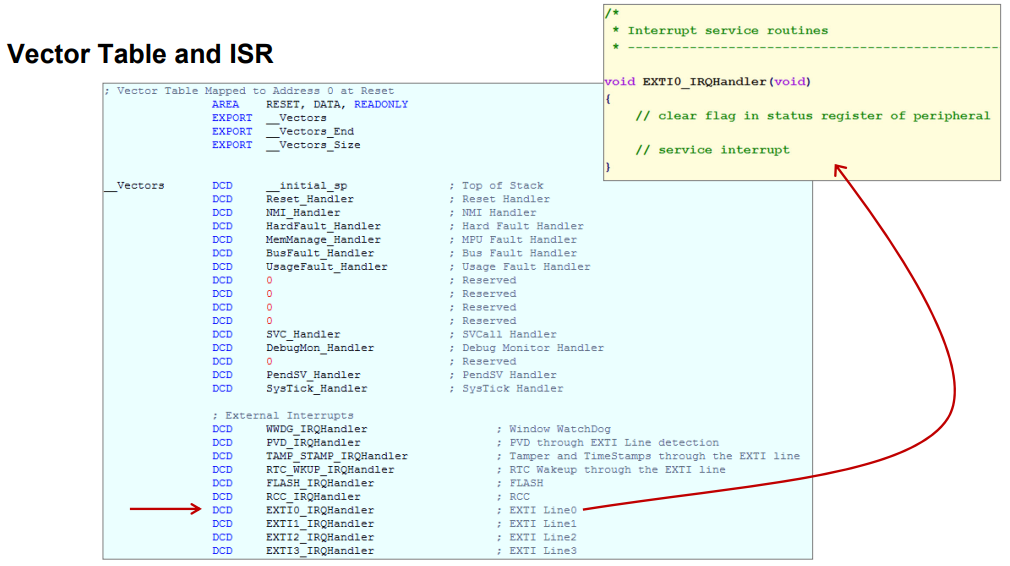
\includegraphics[width=0.9\linewidth]{vectortableisr.png}
\end{concept}

\begin{theorem}{Interrupt flags in Status Registers (SR)} are hardware set and software reset\\
    Software must enable IRQxx line in peripheral\\
    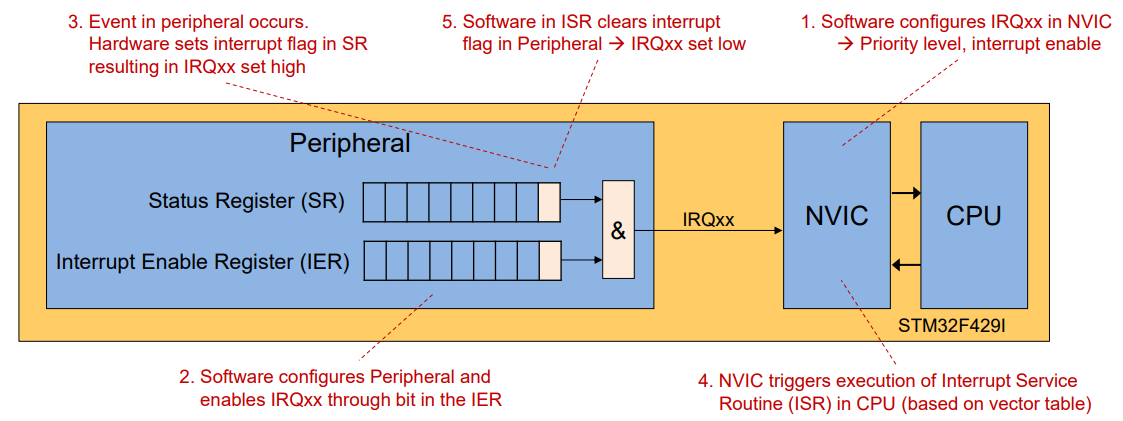
\includegraphics[width=0.9\linewidth]{interruptflagssr.png}
\end{theorem}

\begin{KR}{Configuring Interrupt-Driven I/O}
\paragraph{Step 1: Configure interrupt sources}
Enable specific interrupt sources in peripherals.
\paragraph{Step 2: Configure NVIC}
Set up the Nested Vectored Interrupt Controller for the interrupts.
\paragraph{Step 3: Implement ISRs}
Create Interrupt Service Routines to handle specific events.
\paragraph{Step 4: Enable global interrupts}
Enable the global interrupt flag.

\begin{lstlisting}[language=C, style=basesmol]
// Step 1: Configure SPI interrupt
void configure_spi_interrupt(void) {
    // Enable SPI peripheral clock
    RCC->APB2ENR |= RCC_APB2ENR_SPI1EN;
    
    // Configure SPI parameters
    SPI1->CR1 = SPI_CR1_MSTR | SPI_CR1_SSI | SPI_CR1_SSM;
    
    // Enable SPI TX buffer empty interrupt
    SPI1->CR2 |= SPI_CR2_TXEIE;
    
    // Step 2: Configure NVIC for SPI1
    NVIC_SetPriority(SPI1_IRQn, 2);  // Set priority level
    NVIC_EnableIRQ(SPI1_IRQn);       // Enable interrupt in NVIC
}

// Step 3: Implement SPI1 ISR
void SPI1_IRQHandler(void) {
    // Check if TX buffer empty interrupt
    if (SPI1->SR & SPI_SR_TXE) {
        if (spi_tx_count < spi_tx_length) {
            // Send next byte
            SPI1->DR = spi_tx_buffer[spi_tx_count++];
        } else {
            // Transfer complete, disable interrupt
            SPI1->CR2 &= ~SPI_CR2_TXEIE;
        }
    }
}

// Main function
int main(void) {
    // Initialize system
    system_init();
    
    // Configure SPI interrupt
    configure_spi_interrupt();
    
    // Step 4: Enable global interrupts
    __enable_irq();
    
    // Main loop - can perform other tasks
    while (1) {
        process_system_tasks();
    }
}
\end{lstlisting}
\end{KR}

\raggedcolumns
\columnbreak

\subsection{Interrupt Performance Analysis}

\begin{concept}{Interrupt Performance Metrics}\\
\important{Interrupt-Frequenz} $f_{INT}$ [Hz]: How often does an interrupt occur\\
 Varies from source to source, e.g.:\\
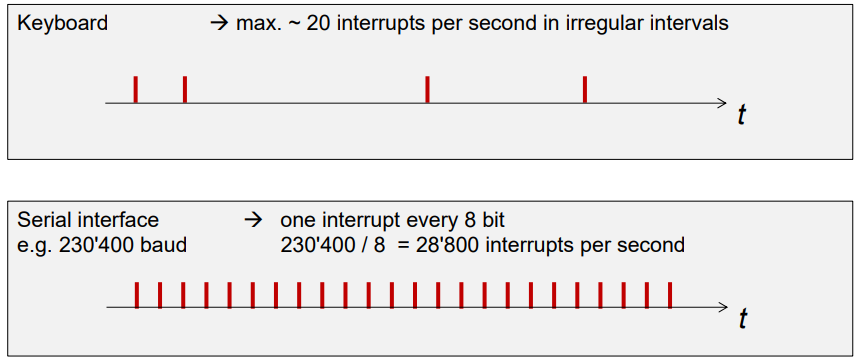
\includegraphics[width=0.6\linewidth]{interruptfrquency.png}

\begin{minipage}{0.7\linewidth}
\important{Interrupt Service Time} $t_{ISR}$ [s]: Required time to process an interrupt\\ (execution time of ISR)\\
    Depends on:
    \begin{itemize}
        \item Number of instructions in ISR
        \item required clock cycles per instruction (CPU architecture)
        \item CPU clock frequency
        \item Time for switching to and returning from ISR
    \end{itemize}
\end{minipage}
\begin{minipage}{0.3\linewidth}
    \vspace{-20mm}
    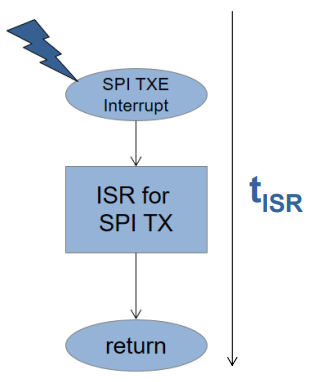
\includegraphics[width=\linewidth]{interruptservicetime.png}
\end{minipage}

\begin{itemize}
    \item \important{Interrupt Latency}: Time between interrupt event and start of ISR execution
    \item \important{System Impact}: Percentage of CPU time spent handling interrupts
\end{itemize}

\end{concept}

\begin{theorem}{Impact of Interrupts on System Performance}\\
\important{Impact} [\%]: Percentage of CPU time used to service interrupts
$$\text{Impact} = f_{INT} \times t_{ISR} \times 100\%$$
    \begin{itemize}
        \item Impact $<$ 100\%: System can handle all interrupts
        \item Impact $>$ 100\%: Some interrupts will not be serviced, data loss possible
    \end{itemize}
$f_{INT}$ and $t_{ISR}$ may vary over time: Average may be ok, but individual interrupt events may still be lost

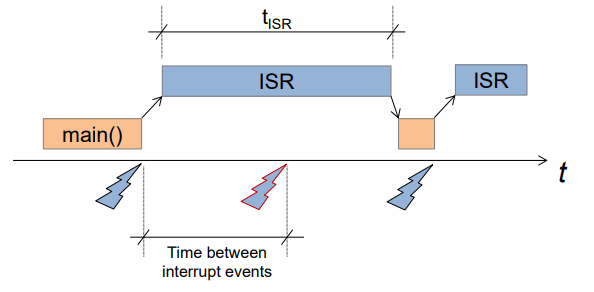
\includegraphics[width=0.6\linewidth]{timebetweeninterruptevents.png}

\textbf{Caution in case of several interrupt sources:}
    \begin{itemize}
        \item Interrupts may occur simultaneously
        \item Impact of all sources must be considered
        \item Critical sources may have higher impact than average
        \item System design must account for worst-case scenarios
    \end{itemize}
    
\end{theorem}

\begin{example}
    \begin{itemize}
    \item Keyboard interrupt: $f_{INT} = 20$ Hz = $20 \frac{1}{s}$, $t_{ISR} = 6$ µs
    $$
    \text{Impact} = 20 \text{ Hz} \times 6 \text{ µs} \times 100\% = 0.012\%
    $$

    \item High-speed serial interface with 230400 Baud: $f_{INT} = \frac{230400}{8} = 28,800$ Hz, $t_{ISR} = 6$ µs
   $$
    \text{Impact} = 28,800 \text{ Hz} \times 6 \text{ µs} \times 100\% = 17.3\%
   $$
\end{itemize}
\end{example}

\mult{2}

\begin{formula}{Interrupt Performance Formulas}

    $$f_{INT} = \frac{\text{data rate [bit/s]}}{\text{buffer size [bit]}}$$

    $$t_{ISR} = \frac{\text{clock cycles}}{\text{CPU-frequency [Hz]}}$$

    $$\text{Impact} = f_{INT} \times t_{ISR} \times 100\%$$
    
    
    \paragraph{Critical Data Rate}
    \begin{itemize}
        \item For 100\% CPU usage: $f_{INT} \times t_{ISR} = 1$
        \item Maximal data rate: $\text{Rate}_{max} = \frac{\text{buffer size}}{t_{ISR}}$
    \end{itemize}
\end{formula}

\begin{example}
    A processor system (1 MHz clock) receives data at 16 kbit/s. The peripheral device can buffer 32 bits. The ISR requires 100 clock cycles.
    \vspace{1mm}\\
    \textbf{Calculate impact:}
    \begin{itemize}
        \item $f_{INT} = \frac{16 \text{ kbit/s}}{32 \text{ bit}} = 500 \text{ Hz}$
        \item $t_{ISR} = \frac{100 \text{ cycles}}{1 \text{ MHz}} = 100 \mu s$
        \item $\text{Impact} = 500 \text{ Hz} \times 100 \mu s \times 100\% = 5\%$
    \end{itemize}
    \vspace{1mm}
    \textbf{Critical data rate for 100\% CPU load:}
    \begin{itemize}
        \item $(x / 32 \text{ bit}) \times 100 \mu s = 1$
        \item $x = \frac{32 \text{ bit}}{100 \mu s} = 320 \text{ kbit/s}$
    \end{itemize}
    \vspace{1mm}
    \textbf{Data loss at 90\% load:}
    \\ ISR time varies depending on instruction and data $\Rightarrow$ peaks can lead to data loss.
\end{example}

\multend

\begin{KR}{Analyzing Interrupt System Performance}
\paragraph{Calculate interrupt frequency}
\begin{itemize}
    \item Identify the source and rate of interrupts
    \item For periodic interrupts, calculate frequency directly
    \item For data-driven interrupts (e.g., serial interface), calculate:
    \begin{itemize}
        \item f$_{INT}$ = data\_rate / data\_size\_per\_interrupt
        \item Example: 9600 baud UART with 8 data bits = 9600/8 = 1200 Hz
    \end{itemize}
\end{itemize}

\paragraph{Determine interrupt service time}
\begin{itemize}
    \item Estimate execution time of the Interrupt Service Routine (ISR)
    \item Include: Context switching time (register saving/restoring), Instruction execution time of the routine itself, Memory access time
    \item Measure or calculate in CPU clock cycles, then convert to time
    \item t$_{ISR}$ = cycles / f$_{CPU}$
\end{itemize}

\paragraph{Calculate system impact}
\begin{itemize}
    \item Percentage of CPU time used by interrupts:
    \item Impact = f$_{INT}$ × t$_{ISR}$ × 100\%
    \item Assess if the impact is acceptable:
    \begin{itemize}
        \item < 10\%: Minimal impact
        \item 10-50\%: Moderate impact
        \item > 50\%: Significant impact, may need optimization
        \item > 90\%: System likely unable to perform other tasks
    \end{itemize}
    \item Check if t$_{ISR}$ > 1/f$_{INT}$ - indicates missed interrupts
\end{itemize}
\end{KR}

\begin{example2}{Interrupt System Analysis}
A processor system running at 1 MHz receives data through a peripheral interface at a rate of 16 kbit/s. The peripheral can buffer 32 bits of data and signals the processor via an interrupt line when the buffer is ready to be read. If the data is not read before the next interrupt, it is lost.
\vspace{1mm}\\
The Interrupt Service Routine (ISR) requires 100 clock cycles on average, including call and return overhead. The system uses no other interrupts.
\vspace{1mm}\\
1. \textbf{Calculate interrupt impact:}
   \begin{itemize}
     \item Interrupt frequency: f$_{INT}$ = 16 kbit/s ÷ 32 bits = 500 Hz
     \item Interrupt service time: t$_{ISR}$ = 100 cycles ÷ 1 MHz = 100 $mu$s
     \item Impact = f$_{INT}$ × t$_{ISR}$ × 100\% = 500 Hz × 100 $mu$s × 100\% = 5\%
   \end{itemize}
   Therefore, interrupts consume 5\% of the CPU's processing time.

2. \textbf{Maximum data rate calculation:}
   \begin{itemize}
     \item For 100\% CPU usage: 1 = f$_{INT}$ × t$_{ISR}$
     \item f$_{INT}$ = 1 ÷ t$_{ISR}$ = 1 ÷ 100 $mu$s = 10,000 Hz
     \item Data rate = f$_{INT}$ × 32 bits = 10,000 × 32 = 320 kbit/s
   \end{itemize}

3. \textbf{Cause of occasional data loss:}
   \begin{itemize}
     \item At 90\% CPU utilization, there should theoretically be enough time to process all interrupts
     \item However, the service time (t$_{ISR}$) is not constant but an average
     \item Some interrupt instances may take longer than the average 100 cycles
     \item When t$_{ISR}$ varies, occasional peaks can exceed the time between interrupts
     \item Result: occasional buffer overflows and data loss
   \end{itemize}
\end{example2}

\raggedcolumns
\columnbreak





\subsection{Interrupt Latency}

\begin{definition}{Interrupt Latency}\\
Interrupt latency is the time between an interrupt event and the first useful instruction execution in the ISR:
\begin{itemize}
    \item \textbf{Hardware Latency}: Time for hardware to detect and signal the event
    \item \textbf{Arbitration Latency}: Time to determine which interrupt to service (if multiple)
    \item \textbf{CPU Latency}: Time to complete current instruction and save context
    \item \textbf{OS/Software Latency}: Additional delays due to software overhead
\end{itemize}
Latency is critical for real-time systems, where guaranteed response times are required.
\begin{itemize}
    \item Range: from about 50 nanoseconds up to several milliseconds
\end{itemize}
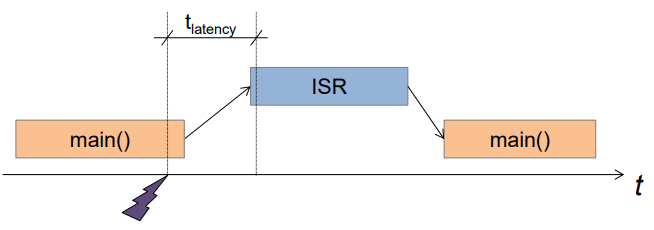
\includegraphics[width=0.7\linewidth]{interruptlatency.png}
\end{definition}

\begin{concept}{Sources of Interrupt Latency}
Several factors contribute to interrupt latency:
\begin{itemize}
    \item \textbf{Current CPU Instruction}:
    \begin{itemize}
        \item Multi-cycle instructions may complete before the interrupt is serviced
        \item Some instructions may be abandoned and restarted (e.g., SDIV/UDIV on Cortex-M3/M4)
        \item Some may be interrupted and resumed (e.g., LDM/STM on Cortex-M3/M4)
    \end{itemize}
    \item \textbf{Disabled Interrupts}:
    \begin{itemize}
        \item Global interrupts may be disabled (CPSID i / CPSIE i)
        \item Specific interrupts may be masked
    \end{itemize}
    \item \textbf{Higher Priority Interrupts}:
    \begin{itemize}
        \item Lower priority interrupts wait until higher priority ones complete
    \end{itemize}
    \item \textbf{Context Saving}:
    \begin{itemize}
        \item Pushing registers to stack
        \item More registers saved means higher latency
    \end{itemize}
    \item \textbf{Cache and Memory Behavior}:
    \begin{itemize}
        \item Cache misses when fetching ISR code
        \item Memory wait states
    \end{itemize}
\end{itemize}
\end{concept}

\begin{corollary}{Response Time}\\
    \textbf{Required response time for a specific event}
    \begin{itemize}
        \item Certain peripherals require fast response times (< 1µs)
        \item Real-time systems, e.g. anti-lock braking system
        \item Cannot be guaranteed if maximum interrupt latency is too high
    \end{itemize}

\textbf{$\mathrm{f}_{\text {INT }}$ too high $\boldsymbol{\rightarrow}$ Too many interrupts}
\begin{itemize}
    \item No CPU cycles left for data processing
    \item System is busy calling ISRs
    \item Neither ISR nor main loop can process any data
    \item Performance of CPU is used only for latencies / context switching
\end{itemize}

\textbf{Fast response times - low latency}
\begin{itemize}
    \item Fast CPU with high clock rate
    \item Low number of clock cycles per instruction
    \item Extremely short polling loops can be fast
    \item Pre-emption with appropriate priorities
    \item Priority levels programmed in NVIC
    \item Real Time OS
\end{itemize}    
\end{corollary}

\begin{theorem}{Latency influenced by hardware (CPU)}
    \begin{itemize}
        \item Different instructions may have different execution times
        \item Multi-cycle instructions on Cortex-M3/M4\\
        \small
        Some (e.g. SDIV/UDIV) are abandoned and restarted after ISR\\
        Some (e.g. LDM/STM) are interrupted and resumed after ISR
    \end{itemize}
    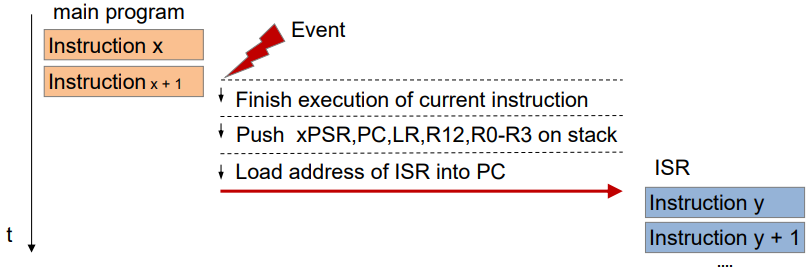
\includegraphics[width=\linewidth]{latencyinfluencedhw.png}
\end{theorem}

\begin{theorem}{Latency influenced by software (code)}
    \begin{itemize}
        \item Saving additional registers on stack
        \item Process ongoing or higher prioritized ISRs
        \item Interrupts may be disabled/masked (CPSID i / CPSIE i)
        \item In case several sources are using the same interrupt line: SW has to use polling to know which peripheral requires servicing
    \end{itemize}
    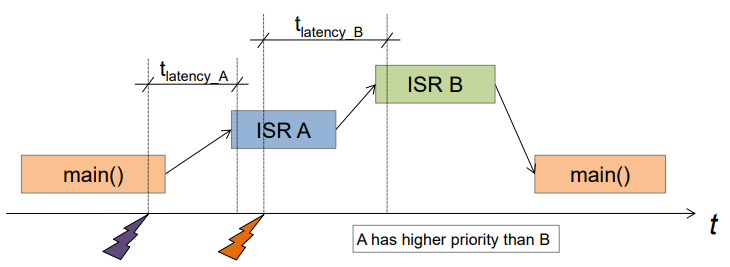
\includegraphics[width=\linewidth]{latencyinfluenesw.png}
\end{theorem}

\raggedcolumns
\columnbreak

\subsection{Pre-emption and Priority}

\begin{concept}{Nested Vector Interrupt Controller (NVIC)}\\
The ARM Cortex-M NVIC provides advanced interrupt handling features:
\begin{itemize}
    \item Supports up to 240 external interrupt sources (IRQs)
    \item Each interrupt can be assigned one of 256 priority levels (processor specific)
    \item Priority-based interrupt preemption
    \item Automatic context saving and restoring
    \item Tail-chaining optimization (reduced latency between ISRs)
    \item Late-arrival handling (higher priority interrupts can overtake pending lower ones)
\end{itemize}
\end{concept}

\begin{definition}{Interrupt Preemption}\\
Preemption allows higher-priority interrupts to interrupt lower-priority ones:
\begin{itemize}
    \item When a higher-priority interrupt occurs during a lower-priority ISR
    \item Current ISR is suspended (context saved)
    \item Higher-priority ISR executes
    \item After completion, lower-priority ISR resumes
\end{itemize}
This ensures that critical interrupts are handled promptly, regardless of other interrupt activity.
\end{definition}

\begin{concept}{Priority-Based Interrupt Handling}\\
Key aspects of priority-based interrupt handling:
\begin{itemize}
    \item \textbf{Priority Assignment}:
    \begin{itemize}
        \item Assign priorities based on time-criticality and importance
        \item Lower numerical values usually indicate higher priority
    \end{itemize}
    \item \textbf{Priority Grouping}:
    \begin{itemize}
        \item Cortex-M supports priority grouping into pre-emption and sub-priority levels
        \item Pre-emption priority determines whether an interrupt can pre-empt another
        \item Sub-priority determines ordering when multiple interrupts of same pre-emption priority occur
    \end{itemize}
    \item \textbf{Priority Inversion}:
    \begin{itemize}
        \item Problem where a high-priority task is indirectly delayed by a low-priority task
        \item Can be mitigated through proper design and priority inheritance protocols
    \end{itemize}
\end{itemize}
\end{concept}

\begin{theorem}{Example Interrup Priorities}
    ISR1 does not pre-empt ISR0, ISR2 pre-empts ISR0
    \begin{itemize}
        \item IRQ0: PL0 = 0x2  (medium priority)
        \item IRQ1: PL1 = 0x3  (lowest priority)
        \item IRQ2: PL2 = 0x1  (highest priority)
    \end{itemize}
    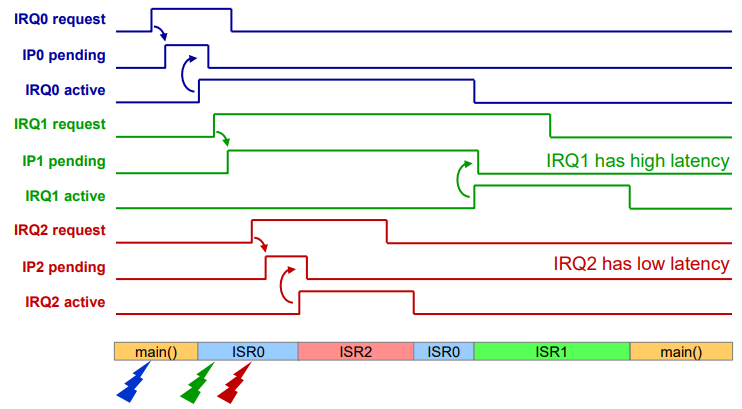
\includegraphics[width=\linewidth]{interruptpriorities.png}
\end{theorem}

\begin{KR}{Configuring Interrupt Priorities}
\paragraph{Step 1: Analyze timing requirements}
Determine which interrupts are most time-critical.
\paragraph{Step 2: Group interrupts by importance}
Create logical groups based on system criticality.
\paragraph{Step 3: Assign priority levels}
Configure NVIC priority registers for each interrupt.
\paragraph{Step 4: Configure priority grouping}
Set priority group using NVIC\_SetPriorityGrouping().

\begin{lstlisting}[language=C, style=basesmol]
// Configure interrupt priorities
void configure_interrupt_priorities(void) {
    // Set priority grouping (4 bits for pre-emption priority, 0 bits for sub-priority)
    NVIC_SetPriorityGrouping(3);
    
    // Critical interrupts (highest priority)
    NVIC_SetPriority(EXTI0_IRQn, 0);      // Emergency stop button
    NVIC_SetPriority(TIM1_UP_IRQn, 1);    // Critical timing control
    
    // Medium priority interrupts
    NVIC_SetPriority(SPI1_IRQn, 4);       // Sensor data acquisition
    NVIC_SetPriority(USART2_IRQn, 5);     // Communication
    
    // Lower priority interrupts
    NVIC_SetPriority(ADC_IRQn, 10);       // Regular ADC sampling
    NVIC_SetPriority(TIM3_IRQn, 11);      // Status LED updates
    
    // Enable the interrupts
    NVIC_EnableIRQ(EXTI0_IRQn);
    NVIC_EnableIRQ(TIM1_UP_IRQn);
    NVIC_EnableIRQ(SPI1_IRQn);
    NVIC_EnableIRQ(USART2_IRQn);
    NVIC_EnableIRQ(ADC_IRQn);
    NVIC_EnableIRQ(TIM3_IRQn);
}
\end{lstlisting}
\end{KR}

\raggedcolumns
\columnbreak

\subsection{Managing Interrupt Latency}

\begin{minipage}{0.6\linewidth}
\begin{definition}{Latency Consistency}
    Some applications can tolerate considerable interrupt latency as long as it is consistent\\
(same amount of latency from one interrupt event to next one)
\vspace{1mm}\\
Example: Measurements with periodic time intervals\\
- Path measurements to detect whether an object is being accelerated, e.g. counting of step pulses on an incremental position encoder for a motor\\
- Works only with a constant time interval
\end{definition}

\begin{concept}{Managing Interrupt Latency}
    High priority interrupts may \\cause high latencies for lower priority interrupts
    \vspace{1mm}\\
\small
Example for high priority ISR\\
- Interrupt triggers reading of input data\\
- Process data\\
- Write to output\\
- Writing may have to wait for output device to become available\\
- E.g. because SPI is still transmitting previous data
\end{concept}
\end{minipage}
\begin{minipage}{0.4\linewidth}
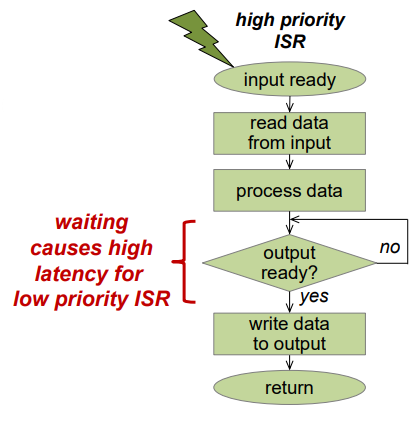
\includegraphics[width=\linewidth]{managinglatency.png}
\end{minipage}

\begin{theorem}{Remedy: Move waiting loop to main program}
    \begin{itemize}
        \item Use queue (FIFO) for decoupling
        \item Makes input ISR short and deterministic
    \end{itemize}
    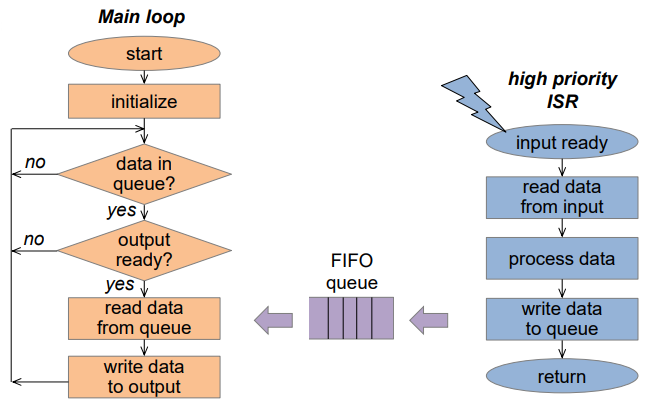
\includegraphics[width=0.6\linewidth]{remedylatency1.png}
    
\end{theorem}

\begin{theorem}{Move non-time-critical work from ISRs to main loop}
    \begin{itemize}
        \item Several ISRs write input data into their dedicated queues
        \item Main loop checks all queues and processes their contents
        \item May result in many tasks in main loop
        \item Not all processing tasks have the same priority
        \item Requires scheduling of tasks
        \item May require real-time OS in case of many ISRs
    \end{itemize}

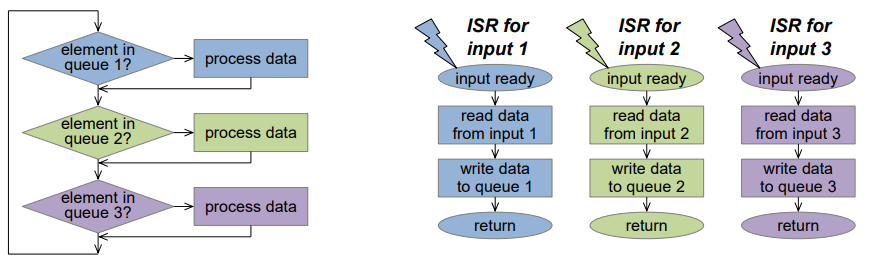
\includegraphics[width=\linewidth]{latencyremedy2.png}
    
\end{theorem}

\begin{KR}{Managing Interrupt Latency in C}
\paragraph{Use interrupt priorities}
Assign appropriate priorities based on timing requirements.
\paragraph{Limit interrupt disable periods}
Minimize sections where interrupts are disabled.
\paragraph{Optimize context switching}
Use processor features that minimize context save/restore.
\paragraph{Preempt lower-priority tasks}
Allow high-priority interrupts to preempt less critical ones.
\paragraph{Move waiting loops to main program}
Don't block inside ISRs waiting for slow peripherals.

\begin{lstlisting}[language=C, style=basesmol]
// Poor: Blocking in ISR
void SPI1_IRQHandler(void) {
    // Read data from input
    input_data = read_input_source();
    
    // Process data
    processed_data = process_data(input_data);
    
    // Wait for output device to be ready (blocking)
    while (!(SPI1->SR & SPI_SR_TXE)) { }
    
    // Write data to output
    SPI1->DR = processed_data;
}

// Better: Queue-based approach
void SPI1_IRQHandler(void) {
    // Read data from input
    input_data = read_input_source();
    
    // Process data
    processed_data = process_data(input_data);
    
    // Add to output queue and return
    queue_add(output_queue, processed_data);
}

// In main loop
void main(void) {
    // Initialize
    system_init();
    
    while (1) {
        // Check if there's data to send and SPI is ready
        if (!queue_empty(output_queue) && (SPI1->SR & SPI_SR_TXE)) {
            // Send next item
            SPI1->DR = queue_get(output_queue);
        }
        
        // Other tasks
        process_system_tasks();
    }
}
\end{lstlisting}
\end{KR}

\begin{KR}{Managing Interrupt Latency}
\paragraph{Understand latency components}
\begin{itemize}
    \item \textbf{Hardware latency:}
    \begin{itemize}
        \item Time for interrupt controller to recognize interrupt
        \item Time to finish current instruction (multi-cycle instructions)
        \item Time to push registers onto stack
    \end{itemize}
    \item \textbf{Software latency:}
    \begin{itemize}
        \item Interrupt disabled periods
        \item Higher priority interrupt processing
        \item Cache misses during ISR execution
    \end{itemize}
\end{itemize}

\paragraph{Measure interrupt latency}
\begin{itemize}
    \item Use an oscilloscope to measure time between:
    \begin{itemize}
        \item Interrupt trigger signal
        \item GPIO pin toggle in ISR
    \end{itemize}
    \item Alternatively, use a timer to capture timestamps:
    \begin{itemize}
        \item Configure timer to capture on interrupt signal
        \item Read timer value at ISR entry
        \item Calculate difference
    \end{itemize}
    \item Measure best-case, worst-case, and average latency
\end{itemize}

\paragraph{Optimize for consistent latency}
\begin{itemize}
    \item Minimize interrupt disable periods
    \begin{itemize}
        \item Keep critical sections short
        \item Use selective interrupt masking instead of global disable
    \end{itemize}
    \item Optimize ISR code
    \begin{itemize}
        \item Minimize stack usage to reduce push/pop operations
        \item Keep ISRs short and efficient
        \item Ensure frequently used data and code are in cache
    \end{itemize}
    \item Use appropriate priorities
    \begin{itemize}
        \item Assign higher priorities to time-critical interrupts
        \item Group interrupts with similar timing requirements
    \end{itemize}
\end{itemize}

\paragraph{Implement deterministic response}
\begin{itemize}
    \item For time-critical operations, consider:
    \begin{itemize}
        \item Polling instead of interrupts if determinism is crucial
        \item Hardware solutions (DMA, dedicated controllers)
        \item Real-time operating system with predictable scheduling
    \end{itemize}
    \item Move processing from ISRs to main loop
    \begin{itemize}
        \item ISR only captures essential data and signals main loop
        \item Use flags, semaphores, or message queues for communication
    \end{itemize}
\end{itemize}
\end{KR}






\subsection{Interrupt-Driven System Design}




\begin{KR}{Designing Efficient Interrupt-Driven Systems}
\paragraph{Choose between polling and interrupts}
\begin{itemize}
    \item \textbf{Use interrupts when:}
    \begin{itemize}
        \item Events occur infrequently or at unpredictable times
        \item System needs to respond to external events quickly
        \item Power efficiency is important (can sleep between events)
        \item Multiple event sources need to be monitored simultaneously
    \end{itemize}
    \item \textbf{Use polling when:}
    \begin{itemize}
        \item Events occur at very high frequency
        \item Absolute determinism is required
        \item Interrupt overhead would be excessive
        \item Extremely low latency is required
    \end{itemize}
\end{itemize}

\paragraph{Design efficient ISRs}
\begin{itemize}
    \item Keep ISRs as short as possible
    \begin{itemize}
        \item Only handle time-critical operations in the ISR
        \item Defer processing to main loop using flags or queues
        \item Avoid complex calculations or I/O operations
    \end{itemize}
    \item Manage shared resources
    \begin{itemize}
        \item Use volatile for variables shared between ISR and main code
        \item Consider atomic operations for simple updates
        \item Implement proper synchronization for complex data structures
    \end{itemize}
    \item Avoid nesting or recursion in ISRs
\end{itemize}

\paragraph{Implement event queues}
\begin{itemize}
    \item Use queue to transfer events from ISRs to main loop
    \begin{itemize}
        \item ISR detects event and enqueues it
        \item Main loop dequeues and processes events
    \end{itemize}
    \item Design queue to be interrupt-safe
    \begin{itemize}
        \item Use atomic operations if available
        \item Consider implementing lock-free algorithms
        \item Size queue appropriately to avoid overflow
    \end{itemize}
    \item Process events in order of importance or arrival
\end{itemize}

\paragraph{Implement event-driven architecture}
\begin{itemize}
    \item Structure code as state machines responding to events
    \item Separate event detection (ISRs) from processing (handlers)
    \item Design for different operating modes
    \begin{itemize}
        \item Normal operation
        \item Power-saving modes
        \item Error handling and recovery
    \end{itemize}
    \item Consider using an RTOS for complex systems
\end{itemize}
\end{KR}



\raggedcolumns
\pagebreak
















\subsubsection{Interrupt-Driven State Machines}

\begin{definition}{Events Trigger Interrupts}\\
    Several Interrupt Service Routines (ISR) enter events into queue
    FSM in main loop reads events from queue

    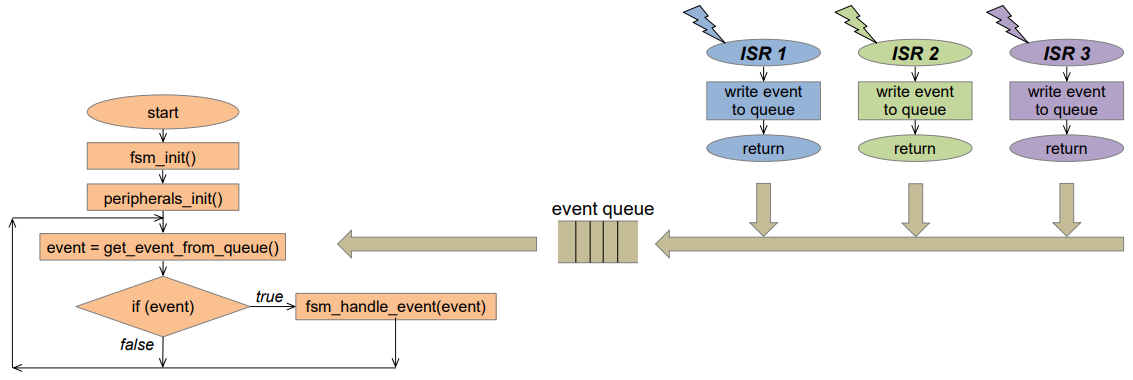
\includegraphics[width=\linewidth]{interruptdrivenfsm.png}
\end{definition}

\begin{concept}{Interrupt-driven Finite State Machine}\\
    Kombination von Interrupt-System und Zustandsautomat:
    \begin{itemize}
        \item ISRs generieren Events und schreiben sie in Queue
        \item FSM in Main Loop liest Events aus Queue
        \item Deterministische Event-Verarbeitung
        \item Saubere Trennung von Interrupt- und Anwendungslogik
    \end{itemize}
\end{concept}

\begin{theorem}{Integrating Interrupts and State Machines}\\
Combining interrupt-driven I/O with state machines creates efficient event-driven systems:
\begin{itemize}
    \item \textbf{Event Queue}: Buffer between ISRs and state machine
    \begin{itemize}
        \item ISRs detect events and add them to queue
        \item Main loop pulls events from queue and feeds state machine
    \end{itemize}
    \item \textbf{ISR Responsibilities}:
    \begin{itemize}
        \item Minimal processing (detect event, capture data)
        \item Add event to queue
        \item Return quickly
    \end{itemize}
    \item \textbf{Main Loop Responsibilities}:
    \begin{itemize}
        \item Pull events from queue
        \item Process events through state machine
        \item Handle longer-duration processing
    \end{itemize}
\end{itemize}
\end{theorem}


\begin{KR}{Implementing Interrupt-Driven FSM}\\
\textbf{Step 1: Create event queue}
Implement a buffer to store events from ISRs.

\textbf{Step 2: Implement ISRs}
Keep ISRs short, just capturing events and adding to queue.

\textbf{Step 3: Implement state machine}
Create state machine logic to process events from queue.

\textbf{Step 4: Connect with main loop}
Pull events from queue and feed to state machine in main loop.

\begin{lstlisting}[language=C, style=basesmol]
// Define event types and queue
typedef enum {
    EVENT_BUTTON_PRESS,
    EVENT_TIMEOUT,
    EVENT_SENSOR_TRIGGER,
    EVENT_NO_EVENT
} event_t;

#define EVENT_QUEUE_SIZE 16
event_t event_queue[EVENT_QUEUE_SIZE];
int queue_head = 0;
int queue_tail = 0;
int queue_count = 0;
// Add event to queue (called from ISRs)
void queue_add_event(event_t event) { 
    if (queue_count < EVENT_QUEUE_SIZE) {
        event_queue[queue_tail] = event;
        queue_tail = (queue_tail + 1) % EVENT_QUEUE_SIZE;
        queue_count++;
    }
}
// Get event from queue (called from main loop)
event_t queue_get_event(void) { 
    event_t event = EVENT_NO_EVENT;
    if (queue_count > 0) {
        event = event_queue[queue_head];
        queue_head = (queue_head + 1) % EVENT_QUEUE_SIZE;
        queue_count--;
    }
    return event;
}

void EXTI0_IRQHandler(void) { // Button interrupt handler
    // Check if EXTI0 interrupt occurred
    if (EXTI->PR & EXTI_PR_PR0) {
        queue_add_event(EVENT_BUTTON_PRESS); // Add button press event to queue
        EXTI->PR = EXTI_PR_PR0; // Clear pending bit
    }
}
void TIM2_IRQHandler(void) { // Timer interrupt handler
    if (TIM2->SR & TIM_SR_UIF) {
        queue_add_event(EVENT_TIMEOUT); // Add timeout event to queue
        TIM2->SR &= ~TIM_SR_UIF; // Clear update interrupt flag
    }
}
// Main loop with state machine
int main(void) {
    system_init(); // Initialize system and interrupts
    __enable_irq();
    fsm_init(); // Initialize state machine
    while (1) {
        event_t event = queue_get_event(); // Get event from queue
        if (event != EVENT_NO_EVENT) { 
            fsm_handle_event(event); // Process event with state machine
        }
        process_system_tasks(); // Background tasks
    }
}
\end{lstlisting}
\end{KR}




\begin{example2}{Interrupt-Driven UART Communication System}\\
Design an interrupt-driven communication system with the following requirements:
\begin{itemize}
    \item UART interface operating at 115200 baud, 8N1 format
    \item Must handle both transmit and receive operations
    \item System should never lose incoming data
    \item Main application should not be blocked by I/O operations
    \item CPU runs at 72 MHz and has other tasks to perform
\end{itemize}

\tcblower

The system will use an interrupt-driven approach with queues to handle UART communication efficiently:

 \textbf{System architecture:}
   \begin{itemize}
     \item Receive interrupt (RXNE) to handle incoming data
     \item Transmit interrupt (TXE) to send outgoing data
     \item Circular buffers for both TX and RX data
     \item Non-blocking API for the main application
   \end{itemize}

\textbf{Key design elements:}
   \begin{itemize}
     \item \textbf{Circular buffers:} Efficient for handling serial data; no memory copying required
     \item \textbf{Non-blocking API:} Main application can send/receive without waiting
     \item \textbf{Interrupt-driven:} Minimal CPU overhead, responds quickly to data
     \item \textbf{Buffer size is power of 2:} Enables efficient masking for wrap-around
     \item \textbf{Buffer management:} Checks for full/empty conditions to prevent data loss
     \item \textbf{Critical sections:} Protect shared buffer access between ISR and main code
   \end{itemize}

 \textbf{Performance analysis:}
   \begin{itemize}
     \item At 115200 baud, 8N1:
     \begin{itemize}
       \item 1 start bit + 8 data bits + 1 stop bit = 10 bits per byte
       \item Byte rate = 115200/10 = 11520 bytes per second
       \item Time between bytes = 1/11520 $\approx$ 87 $mu$s
     \end{itemize}
     \item With a 256-byte buffer:
     \begin{itemize}
       \item Buffer can hold 256 × 87 $mu$s $\approx$ 22 ms of data
       \item Sufficient for main loop to process data even with other tasks
     \end{itemize}
     \item ISR execution time:
     \begin{itemize}
       \item At 72 MHz, reading a byte and storing it takes ~10 cycles
       \item ISR overhead (entry/exit) ~20 cycles
       \item Total ~30 cycles = 0.42 $mu$s
       \item Impact = 0.42 $mu$s / 87 $mu$s $\approx$ 0.5\% of CPU time
     \end{itemize}
   \end{itemize}

This design provides an efficient, interrupt-driven UART interface that meets all requirements with minimal CPU overhead.

\end{example2}

\begin{example2}{Interrupt-Driven UART Communication System (continued)}

\textbf{Implementation:}

\begin{lstlisting}[language=C, style=basesmol]
#include <stdint.h>
#include <stdbool.h>
// Buffer size must be power of 2 for efficient wrap-around
#define UART_BUFFER_SIZE 256
#define UART_BUFFER_MASK (UART_BUFFER_SIZE - 1)
// Circular buffer structure
typedef struct {
    volatile uint8_t data[UART_BUFFER_SIZE];
    volatile uint16_t head;
    volatile uint16_t tail;
} circular_buffer_t;
// Global buffers
static circular_buffer_t rx_buffer = {0};
static circular_buffer_t tx_buffer = {0};
static volatile bool tx_busy = false;
// Function prototypes
void uart_init(uint32_t baudrate);
bool uart_send_byte(uint8_t data);
bool uart_send_data(const uint8_t* data, uint16_t length);
bool uart_read_byte(uint8_t* data);
uint16_t uart_available(void);
void uart_flush(void);
// External hardware functions
extern void uart_hw_init(uint32_t baudrate);
extern void uart_hw_send_byte(uint8_t data);
extern uint8_t uart_hw_read_byte(void);
extern bool uart_hw_tx_empty(void);
extern bool uart_hw_rx_ready(void);
extern void uart_hw_enable_tx_interrupt(bool enable);
extern void uart_hw_enable_rx_interrupt(bool enable);

// Buffer operations
static bool buffer_is_full(const circular_buffer_t* buffer) {
    return ((buffer->head + 1) & UART_BUFFER_MASK) == buffer->tail;
}

static bool buffer_is_empty(const circular_buffer_t* buffer) {
    return buffer->head == buffer->tail;
}

static bool buffer_push(circular_buffer_t* buffer, uint8_t data) {
    uint16_t next_head = (buffer->head + 1) & UART_BUFFER_MASK;
    
    if (next_head == buffer->tail) {
        return false; // Buffer full
    }
    
    buffer->data[buffer->head] = data;
    buffer->head = next_head;
    return true;
}

static bool buffer_pop(circular_buffer_t* buffer, uint8_t* data) {
    if (buffer->head == buffer->tail) {
        return false; // Buffer empty
    }
    
    *data = buffer->data[buffer->tail];
    buffer->tail = (buffer->tail + 1) & UART_BUFFER_MASK;
    return true;
}

static uint16_t buffer_count(const circular_buffer_t* buffer) {
    return (buffer->head - buffer->tail) & UART_BUFFER_MASK;
}
\end{lstlisting}
\end{example2}

\begin{example2}{Interrupt-Driven UART Communication System (continued)}
\begin{lstlisting}[language=C, style=basesmol]
// UART initialization
void uart_init(uint32_t baudrate) {
    // Initialize hardware
    uart_hw_init(baudrate);
    
    // Reset buffers
    rx_buffer.head = rx_buffer.tail = 0;
    tx_buffer.head = tx_buffer.tail = 0;
    tx_busy = false;
    
    // Enable receive interrupt
    uart_hw_enable_rx_interrupt(true);
    // Transmit interrupt will be enabled when data is available
}

// Send a single byte (non-blocking)
bool uart_send_byte(uint8_t data) {
    bool success;
    bool start_transmission = false;
    
    // Critical section: disable interrupts
    __disable_irq();
    
    success = buffer_push(&tx_buffer, data);
    
    // If TX is not busy and we successfully added data, start transmission
    if (success && !tx_busy) {
        start_transmission = true;
        tx_busy = true;
    }
    
    // End critical section
    __enable_irq();
    
    if (start_transmission) {
        uart_hw_enable_tx_interrupt(true);
    }
    
    return success;
}

// Send multiple bytes (non-blocking)
bool uart_send_data(const uint8_t* data, uint16_t length) {
    for (uint16_t i = 0; i < length; i++) {
        if (!uart_send_byte(data[i])) {
            return false; // Buffer full
        }
    }
    return true;
}

// Read a single byte (non-blocking)
bool uart_read_byte(uint8_t* data) {
    return buffer_pop(&rx_buffer, data);
}

// Get number of bytes available to read
uint16_t uart_available(void) {
    return buffer_count(&rx_buffer);
}
\end{lstlisting}
\end{example2}

\begin{example2}{Interrupt-Driven UART Communication System (continued)}
\begin{lstlisting}[language=C, style=basesmol]
// Flush TX buffer
void uart_flush(void) {
    // Wait until TX buffer is empty
    while (!buffer_is_empty(&tx_buffer)) {
        __NOP(); // No operation - just wait
    }
    
    // Wait until last byte is transmitted
    while (tx_busy) {
        __NOP();
    }
}

// RX interrupt handler
void UART_RX_IRQHandler(void) {
    if (uart_hw_rx_ready()) {
        uint8_t data = uart_hw_read_byte();
        
        // If buffer full, data will be lost
        buffer_push(&rx_buffer, data);
    }
}

// TX interrupt handler
void UART_TX_IRQHandler(void) {
    if (uart_hw_tx_empty()) {
        uint8_t data;
        
        if (buffer_pop(&tx_buffer, &data)) {
            // Send next byte
            uart_hw_send_byte(data);
        } else {
            // No more data, disable TX interrupt
            uart_hw_enable_tx_interrupt(false);
            tx_busy = false;
        }
    }
}

// Example usage in main application
void main(void) {
    // Initialize UART
    uart_init(115200);
    
    // Main loop
    while (1) {
        // Check for received data
        if (uart_available() > 0) {
            uint8_t data;
            uart_read_byte(&data);
            
            // Process received data
            process_data(data);
            
            // Echo back
            uart_send_byte(data);
        }
        
        // Perform other tasks
        other_application_tasks();
    }
}
\end{lstlisting}
\end{example2}

\begin{example2}{Interrupt-Driven FSM Using Timer Interrupts}
Implement a button-controlled LED system with debouncing using timer interrupts.
\tcblower
The system has three states:\\
- OFF: LED is off\\
- ON: LED is on at full brightness\\
- BLINK: LED is blinking
\vspace{1mm}\\
Events:\\
- SHORT\_PRESS: Button pressed briefly\\
- LONG\_PRESS: Button held for >1 second\\
- BLINK\_TIMER: Timer for blinking

\begin{lstlisting}[language=C, style=basesmol]
// Event definitions
typedef enum {
    EVENT_NONE,
    EVENT_SHORT_PRESS,
    EVENT_LONG_PRESS,
    EVENT_BLINK_TIMER
} event_t;

// State definitions
typedef enum {
    STATE_OFF,
    STATE_ON,
    STATE_BLINK
} state_t;

// Global variables
volatile event_t event_queue[10];
volatile uint8_t queue_head = 0;
volatile uint8_t queue_tail = 0;
volatile uint8_t queue_count = 0;
volatile state_t current_state = STATE_OFF;
volatile uint32_t button_press_time = 0;
volatile uint8_t button_released = 1;

// Button interrupt handler (EXTI0)
void EXTI0_IRQHandler(void) {
    uint32_t current_time = HAL_GetTick();
    
    if (EXTI->PR & EXTI_PR_PR0) {
        if (GPIOA->IDR & GPIO_PIN_0) {
            if (!button_released) {
                uint32_t press_duration = current_time - button_press_time;
                if (press_duration > 1000) { // Long press (>1s)
                    if (queue_count < 10) {
                        event_queue[queue_tail] = EVENT_LONG_PRESS;
                        queue_tail = (queue_tail + 1) % 10;
                        queue_count++;
                    }
                } else if (press_duration > 50) { // Short press (debounced)
                    if (queue_count < 10) {
                        event_queue[queue_tail] = EVENT_SHORT_PRESS;
                        queue_tail = (queue_tail + 1) % 10;
                        queue_count++;
                    }
                }
                button_released = 1;
            }
        } else { // Button pressed
            button_press_time = current_time;
            button_released = 0;
        }
        EXTI->PR = EXTI_PR_PR0; // Clear pending bit
    }
}
\end{lstlisting}
\end{example2}

\begin{example2}{Interrupt-Driven FSM Using Timer Interrupts (continued)}
\begin{lstlisting}[language=C, style=basesmol]
// Timer interrupt for blinking (TIM3)
void TIM3_IRQHandler(void) {
    if (TIM3->SR & TIM_SR_UIF) {
        if (queue_count < 10) { // Add blink timer event to queue
            event_queue[queue_tail] = EVENT_BLINK_TIMER;
            queue_tail = (queue_tail + 1) % 10;
            queue_count++;
        }
        TIM3->SR &= ~TIM_SR_UIF; // Clear update interrupt flag
    }
}
// State machine handler
void fsm_handle_event(event_t event) {
    switch (current_state) {
        case STATE_OFF:
            if (event == EVENT_SHORT_PRESS) {
                GPIOC->BSRR = GPIO_PIN_13;
                current_state = STATE_ON; // Turn on LED
                TIM3->CR1 &= ~TIM_CR1_CEN; // Disable blink timer
            } else if (event == EVENT_LONG_PRESS) {
                GPIOC->BSRR = GPIO_PIN_13; // Start blinking
                current_state = STATE_BLINK;
                TIM3->CR1 |= TIM_CR1_CEN; // Enable blink timer
            }
            break;
        case STATE_ON:
            if (event == EVENT_SHORT_PRESS) {
                GPIOC->BSRR = (GPIO_PIN_13 << 16); 
                current_state = STATE_OFF; // Turn off LED
            } else if (event == EVENT_LONG_PRESS) {
                current_state = STATE_BLINK; // Start blinking
                TIM3->CR1 |= TIM_CR1_CEN; // Enable blink timer
            }
            break;
        case STATE_BLINK:
            if (event == EVENT_BLINK_TIMER) {
                GPIOC->ODR ^= GPIO_PIN_13; // Toggle LED
            } else if (event == EVENT_SHORT_PRESS) {
                GPIOC->BSRR = (GPIO_PIN_13 << 16); // Turn off LED and blinking
                current_state = STATE_OFF;
                TIM3->CR1 &= ~TIM_CR1_CEN; // Disable blink timer
            }
            break;
    }
}
// Main function
int main(void) {
    system_init(); // Initialize hardware
    // Configure EXTI for button
    // Configure TIM3 for blinking (500ms period)
    // Enable interrupts
    while (1) {
        // Get and process events
        if (queue_count > 0) {
            event_t event;
            // Disable interrupts to access queue
            __disable_irq();
            event = event_queue[queue_head];
            queue_head = (queue_head + 1) % 10;
            queue_count--;
            __enable_irq();
            // Handle event
            fsm_handle_event(event);
        }
        // System can enter low-power mode here
        // when queue is empty
    }
}
\end{lstlisting}
\end{example2}

\begin{example2}{Interrupt Latency Optimization and ADC}\\
A microcontroller-based system needs to sample an analog signal at precise 100 µs intervals. The current implementation uses Timer1 to generate interrupts every 100 µs, and the ISR reads the ADC. Measurements show that the interrupt latency varies between 5-20 µs, causing jitter in the sampling.

Design an improved solution to minimize sampling jitter, explaining your approach and implementation.

\tcblower
\paragraph{Solution:}

The goal is to reduce sampling jitter by minimizing variations in the time between the timer interrupt and ADC sampling. Here's an improved solution:

\textbf{Hardware-triggered ADC approach:}

1. \textbf{Use timer to trigger ADC directly:}
   \begin{itemize}
     \item Configure Timer1 to generate a trigger signal every 100 µs
     \item Connect this trigger to the ADC hardware trigger input
     \item Configure the ADC to start conversion automatically on timer trigger
     \item Use DMA to transfer ADC results to memory without CPU intervention
   \end{itemize}

2. \textbf{Implementation details:}
\begin{lstlisting}[language=C, style=basesmol]
// Configure Timer1
void configure_timer(void) {
    // Enable clock for Timer1
    RCC->APB2ENR |= RCC_APB2ENR_TIM1EN;
    
    // Set prescaler and period for 100 microsecond interval
    TIM1->PSC = (SystemCoreClock / 1000000) - 1;  // 1 microsecond timer ticks
    TIM1->ARR = 100 - 1;  // 100 microsecond period
    
    // Configure timer to generate trigger output
    TIM1->CR2 &= ~TIM_CR2_MMS;
    TIM1->CR2 |= TIM_CR2_MMS_1;  // Update event as trigger output
    
    // Enable timer
    TIM1->CR1 |= TIM_CR1_CEN;
}

// Configure ADC with timer trigger
void configure_adc(void) {
    // Enable clocks for ADC and GPIO
    RCC->APB2ENR |= RCC_APB2ENR_ADC1EN;
    RCC->AHB1ENR |= RCC_AHB1ENR_GPIOAEN;
    
    // Configure GPIO pin as analog input
    GPIOA->MODER |= GPIO_MODER_MODER0;  // PA0 as analog
    
    // Configure ADC for timer trigger
    ADC1->CR2 |= ADC_CR2_EXTEN_0;        // Enable external trigger on rising edge
    ADC1->CR2 |= ADC_CR2_EXTSEL_3;       // Select Timer1 TRGO as trigger
    
    // Configure single conversion on channel 0
    ADC1->SQR3 = 0;  // Channel 0 as first conversion
    ADC1->SQR1 = 0;  // 1 conversion
    
    // Enable DMA for ADC
    ADC1->CR2 |= ADC_CR2_DMA;
    
    // Enable ADC
    ADC1->CR2 |= ADC_CR2_ADON;
}

\end{lstlisting}
\end{example2}

\begin{example2}{Interrupt Latency Optimization and ADC (continued)}
\begin{lstlisting}[language=C, style=basesmol]

// Configure DMA for ADC
void configure_dma(uint16_t* buffer, uint32_t buffer_size) {
    // Enable DMA clock
    RCC->AHB1ENR |= RCC_AHB1ENR_DMA2EN;
    
    // Configure DMA stream
    DMA2_Stream0->CR &= ~DMA_SxCR_EN;  // Disable DMA during config
    
    DMA2_Stream0->PAR = (uint32_t)&ADC1->DR;       // Source: ADC data register
    DMA2_Stream0->M0AR = (uint32_t)buffer;         // Destination: buffer
    DMA2_Stream0->NDTR = buffer_size;              // Number of data items
    
    DMA2_Stream0->CR &= ~DMA_SxCR_DIR;             // Peripheral to memory
    DMA2_Stream0->CR |= DMA_SxCR_CIRC;             // Circular mode
    DMA2_Stream0->CR |= DMA_SxCR_PSIZE_0;          // Peripheral size: 16 bits
    DMA2_Stream0->CR |= DMA_SxCR_MSIZE_0;          // Memory size: 16 bits
    DMA2_Stream0->CR |= DMA_SxCR_PL_1;             // Priority: high
    
    // Enable DMA
    DMA2_Stream0->CR |= DMA_SxCR_EN;
}

// Main application
int main(void) {
    // Sample buffer
    uint16_t adc_buffer[1000];
    
    // Configure peripherals
    configure_timer();
    configure_adc();
    configure_dma(adc_buffer, 1000);
    
    // Process samples in background
    while (1) {
        // Process captured samples from adc_buffer
        // Buffer is continuously updated by DMA
    }
}
\end{lstlisting}

3. \textbf{Advantages of this approach:}
   \begin{itemize}
     \item Eliminates interrupt latency completely from the sampling process
     \item Hardware triggers ADC directly with precise timing
     \item DMA transfers data without CPU intervention
     \item CPU is free to process samples when available
     \item Sampling jitter reduced to hardware timing accuracy (typically sub-µs)
   \end{itemize}

4. \textbf{Alternative approaches:}
   \begin{itemize}
     \item If hardware triggering is not available, optimize the ISR:
     \begin{itemize}
       \item Set ISR to highest priority
       \item Disable all other interrupts during the ISR
       \item Make the ISR as short as possible (just start ADC)
       \item Use a state variable to track if previous conversion completed
     \end{itemize}
     \item Use a high-precision external timer dedicated to ADC triggering
   \end{itemize}

This solution eliminates software-induced jitter by leveraging hardware synchronization between the timer and ADC, providing the precise 100 µs sampling interval required.
\end{example2}